%\section{Protocol} \fxnote{Did we want to add something about asking them about the pain after each methods? or what did we discuss about this}
%This protocol will describe the present study, which consist of two experiments testing pain tolerance and pain threshold after practicing mindfulness meditation or after not practicing mindfulness meditation. 

\section{Purpose}
%The treatment of chronic pain has constraints, as the treatments are only relieving the pain instead of curing the pain. Another issue is that some of these treatments, example medication, have side effect, as described in \secref{sec:treatment}. 
%There is alternative to medication such as yoga, hypnosis and physical therapy, psychological therapy and chiropractor, which have shown to have an influence on relieving pain. But these treatments are often used in combination with pharmaceutical treatment. Furthermore, most of these alternative require an external person to apply, which can result in high costs, as mention in \secref{sec:treatment}.
%An alternative to the present treatment is mindfulness meditation, which have shown an effect on relieving conditions as stress, depression and  anxiety through the ability to enhance emotion regulation, cognitive control, acceptance and positive mood, as described in \secref{sec:SOTA}. 
%Different studies have shown that practicing meditation have an effect on reliving pain. However, these studies have most often investigated long-term mindfulness meditation for patient with eater chronic pain or low back pain. There is a limit on studies that have investigated short-term in patient with neck pain, why this could be interesting to investigate further, as approximately 25\% of the chronic pain patients suffer from this condition. In order to investigated the influence of mindfulness meditation on pain threshold and pain tolerance for people with neck pain following hypothesis is proposed:

Approximately 375 million people suffer from chronic neck pain. The primary treatment for those patients is medication. But medication has side effects, as described in \secref{sec:treatment}.  Besides medication, alternative treatment methods are used, often in combination with medication. For example physical therapy, chiropractor or psychological therapy showed a positive influence on pain relief. Most of the alternative treatment methods are related with high costs, because they require a specialist for the application. Whereas mindfulness meditation can be practiced alone. Hence a lot of studies focused on the ability of mindfulness meditation to relieve pain.
As mentioned in \secref{sec:SOTA}, there are not many studies which show the effect of mindfulness meditation on chronic neck pain. Since a lot of people suffer from chronic neck pain this study investigates the influence of mindfulness meditation on neck pain. %Pain levels of chronic pain patients are not very easy to access and to quantify, therefore pressure pain was applied with an algometer on healthy subjects, 

%Pain levels of chronic pain patients are not very easy to access and to quantify because the pain is neuropathic and the assessment is multidimensional and the experience of pain is subjective. Therefore, in order to get some quantifiable measures on pain to clarify if mindfulness meditation will have an effect on sensitivity of pain, acute pain in the form of pressure pain was applied to healthy subjects. If the pressure pain tolerance is increased, after practicing mindfulness meditation, in the upper trapezius it might also have an effect on pain in other body parts. And if it is possible to show an effect on acute pain due to an increase in the tolerance on healthy subjects it might also be possible to help relieving pain in chronic pain patients. On basis of this the study wants to test the following hypothesis:

***** This part should be more convincing ****
Pain levels of chronic pain patients are not very easy to access and to quantify because the assessment of neuropathic pain is multidimensional and the experience of chronic pain is subjective. Also variation of the patients' pain from day to day and throughout the day makes it difficult to get reliable and comparable  values of the pain levels of these patients. Therefore acute pressure pain was applied with an algometer to healthy subjects to get quantifiable values of pain and test the following hypothesis: 
*** Until here ***


\textit{Short-term mindfulness meditation practice increases the pressure pain threshold and the pressure pain tolerance in the upper trapezius.}

%\vspace{-.5cm}
%\begin{itemize}
%\item Short-term mindfulness meditation increases the pressure pain threshold and the pressure pain tolerance.
%\end{itemize}

\section{Subjects}
%Forty healthy subjects were recruited for the experiment, 20 males (M) and 20 females (F) with a mean age $\pm$XX. A homogeneous group of participants were enrolled in order to limit the amount of variables in the study. For insuring this, specific inclusion and exclusion criteria have been formed for this experiment. 
40 healthy subjects were recruited for the experiment, 20 males (M) and 20 females
(F) with a mean age of XX$\pm$XX years. To get a homogeneous group of participants, specific inclusion and exclusion criteria were  formed for this experiment.

\textbf{Inclusion criteria:}
\vspace{-.5cm}
\begin{itemize}
	\item Healthy
	\vspace{-.3cm}
	\item Age between 20 and 30 years
	\vspace{-.3cm}
	\item Normal BMI (F: 19-24 M: 20-25)
	\vspace{-.3cm}
	\item Must have time to meditate for 5 days, 20 minutes per day.
\end{itemize}

\textbf{Exclusion criteria:}
\vspace{-.5cm}
\begin{itemize}
	\item Ongoing meditation practice 
	\vspace{-.3cm}
	\item Pregnancy 
	\vspace{-.3cm}
	\item Neurological, musculoskeletal or mental illness
	\vspace{-.3cm}
	\item Abusive drug or alcohol use \fxnote{Think about this 'abusive'}
		\vspace{-.3cm}
			\item Medication with antidepressant or analgesic properties
\vspace{-.3cm}
	\item Lack of ability to cooperate
\end{itemize}

\vspace{-.5cm}
%Furthermore, is it not necessary that subjects believe in the effect of mindfulness meditation.\fxnote{I don't know about this sentence, i think it does not fit in here. Maybe it is more something we should write for the participants or could we put it in as one of our criteria?.}

\section{Study design} 
%For this particular experiment a parallel study was conducted. The subjects recruited for the experiment were randomly assigned in two different groups, the control group or the treatment group, with a equal amount of female and males in the groups. The control group consisted of twenty subjects no meditation. The treatment group consisted of twenty subjects meditation. The structure of the study design is illustrated on \figref{fig:studydesign}. 
For this particular experiment a parallel study was conducted. The subjects, recruited for the experiment, were randomly assigned in two different groups. Whereby an equal amount of females and males were assigned in the control group and the treatment group. The treatment group was measured before and after the intervention, which was the practice of mindfulness meditation. To ensure that a measured effect was not due to habituation to the measurement, a control group was measured with the same time difference. The structure of the study design is illustrated on \figref{fig:studydesign}.

\begin{figure}[H]
	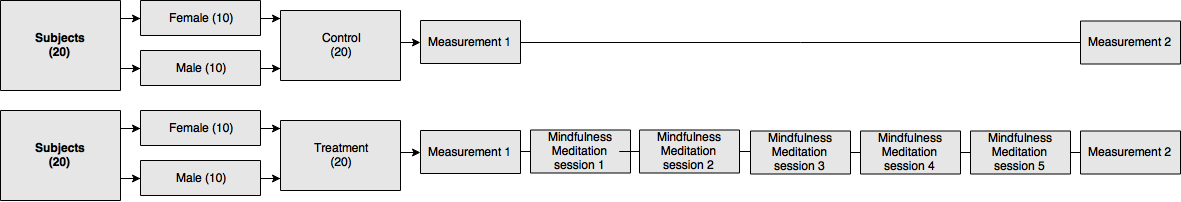
\includegraphics[width=1\textwidth]{figures/studydesign.png} 
	\caption{Parallel study design.}
	\label{fig:studydesign}  
\end{figure}  

%There will be seven to eight days between the measurements. The treatments groups start practicing mindfulness meditation three or four days after the first measurement and will then practice mindfulness meditation for five days and will on the last day of meditation be measured again.

%\section{Setup}
%The Pressure Pain Threshold (PPT), defined as the pressure at which the sensation changed from pressure to pain, has been recognized as an effective and reliable way to quantify pain measures. In this study PPT was measured using Wagner Force Ten$^{TM}$ Digital force Gage. PPT were measured in the upper trapezius. Testing points were marked to ensure reliable and rapid location during the experimental procedure. 
%The algometer was applied four times, two on the left side and two on the right side of the upper trapezius, and the average of the registrations was filed. The subjects had a 5 minutes resting time between measurements. PPT values were measured two times, the first day of the study and after 5 days since the first measure.

%\subsubsection{Mindfulness meditation}
%The treatment group should do guided meditation for 30 minutes in small groups for 5 days. On the first day the mediators would be giving a short introduction to mindfulness meditation. During the meditation the subjects would be in a sitting position with the face  away from the other subjects, to assure that they would not get distracted. 


\section{Procedure}
First of all, general information about the subjects’ were collected, such as gender, height and weight. Furthermore, information about the experiment was given to the subjects. Measurement points were marked at the upper trapezius on both right and left side, as illustrated on \figref{fig:trapezius} while the subjects lay prone to ensure reliable and rapid location during the experimental procedure. The location of the upper trapezius was determined between the acromion and 7th cervical vertebra for both right and left side. These distances were notated so the same locations could be used for each measurement session. 

\begin{figure}[H]
	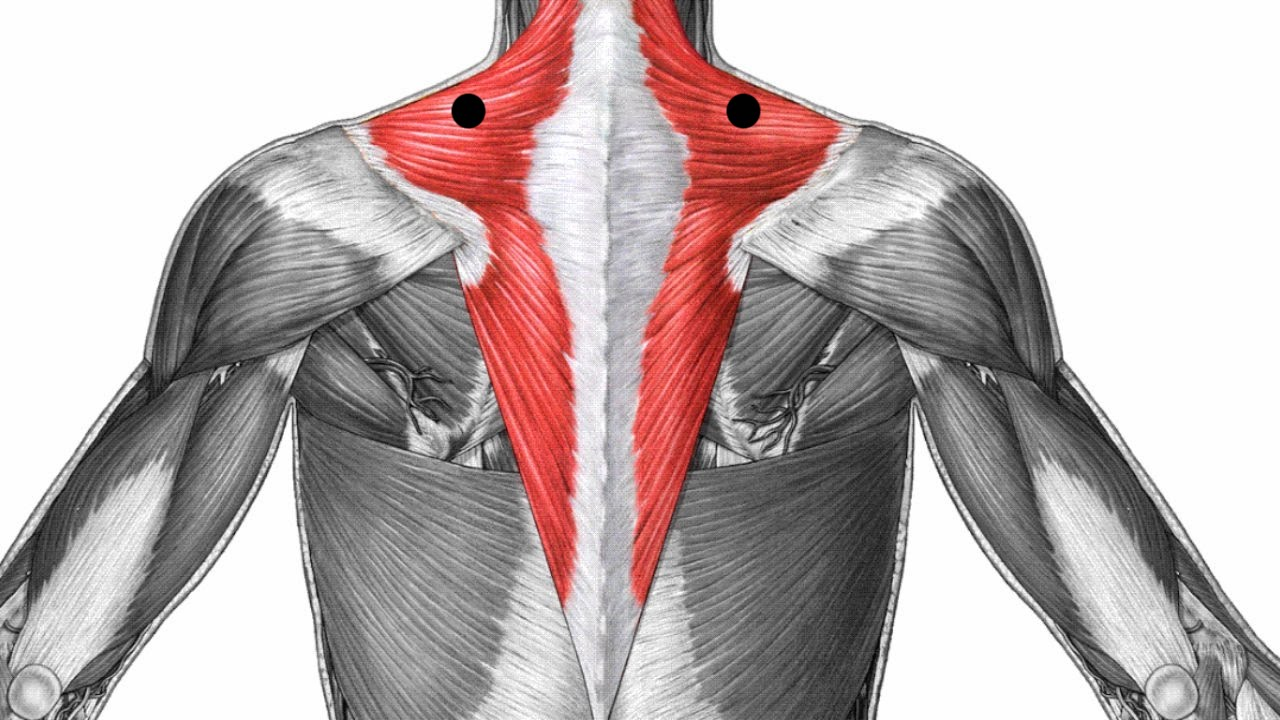
\includegraphics[width=0.5\textwidth]{figures/trapezius} 
	\caption{Measurement on the upper trapezius. The measurement points are mark with black dots.}
	\label{fig:trapezius}  
\end{figure}  

The Pressure Pain Threshold was measured with an algometer (Wagner Force Ten ™  Digital force Gage). Firstly, the algometer was applied until the subject feels it unpleasant and the pain threshold was notated. Secondly, the Pressure Pain Tolerance was measured with the same algometer at the same points and was applied until the subject was feeling to much discomfort to continue.

The same measurement routine was conducted four times, two times on the left upper trapezius and two times on the right upper trapezius. Each measurement was notated and an average of those four measurements was used as for the pain threshold and pain tolerance respectively. To avoid oversensation, the two sides were measured alternately with 1 minute pause in between, so the subjects had a resting time between the measurements on the same side.  

To test the effect of mindfulness meditation on the pressure pain threshold and the pressure pain tolerance, the treatment group practiced 20 minutes mindfulness meditation for 5 consecutive days. To ensure same meditation conditions for all of the subjects, a guided meditation in form of an audio file was used. Furthermore, subjects were told to have the most comfortable position during the meditation.  Additionally a short introduction to mindfulness meditation was provided on the first day. 

The subjects of the control group continued their normal routine.
After the last meditation session of the treatment group the second measurements were conducted. The same time interval between the measurements were used for the subjects of the control group. The second measurement session was conducted likewise the first measurements.



%Then the first measurement was conducted. Thereby Pressure Pain Threshold and Pressure Pain Tolerance were measured with an algometer (Wagner Force Ten ™  Digital force Gage)  in the upper trapezius while the subjects lay prone. The testing points were marked to ensure reliable and rapid location during the experimental procedure. Each, the pressure pain threshold and the pressure pain tolerance, were measured four times, two times on the left upper trapezius and two times on the right  upper trapezius. The average of those four measurements for each variable was used as the value for the first measurement. To avoid oversensation, the two sides were measured alternately with 1 minute pause in between, so  the subjects had a 5 minutes resting time between the measurements on the same side. To test the effect of mindfulness meditation on the pressure pain threshold and the pressure pain tolerance, the treatment group practiced 20 minutes mindfulness meditation for 5 consecutive days. To ensure same meditation conditions for all of the subjects, a guided meditation in form of an audio file was used. Furthermore all meditation sessions took place in the same room. Additionally a short introduction to mindfulness meditation was provided on the first day.
%At the same time, the subjects of the control group continued their normal routine.
%After the last meditation session of the treatment group the second measurement was conducted. The same time interval between the measurements was used for the subjects of the control group. This measurement was conducted likewise the first measurement.


%\subsubsection{Data Analysis}
%To test the hypothesis statistical test was used.The choice of statistically test depends on the the distribution and variance of the dataset. Since, two groups are compared a t-test or Mann-Whitney depending on the distribution. If the data is normal distributed parametric a t-test will be used otherwise a the non-parametric test Mann-Whitney will be used. 